\section{Results}
\subsection{Contours}
Images show contours of pressure and velocity around the car. It is able to see high pressure on the top of aerodynamic elements and negative pressure - under the elements. This difference generate down force which is useful in turns.
\begin{figure}[h!]
	\centering
    \begin{subfigure}[b]{0.48\textwidth}
    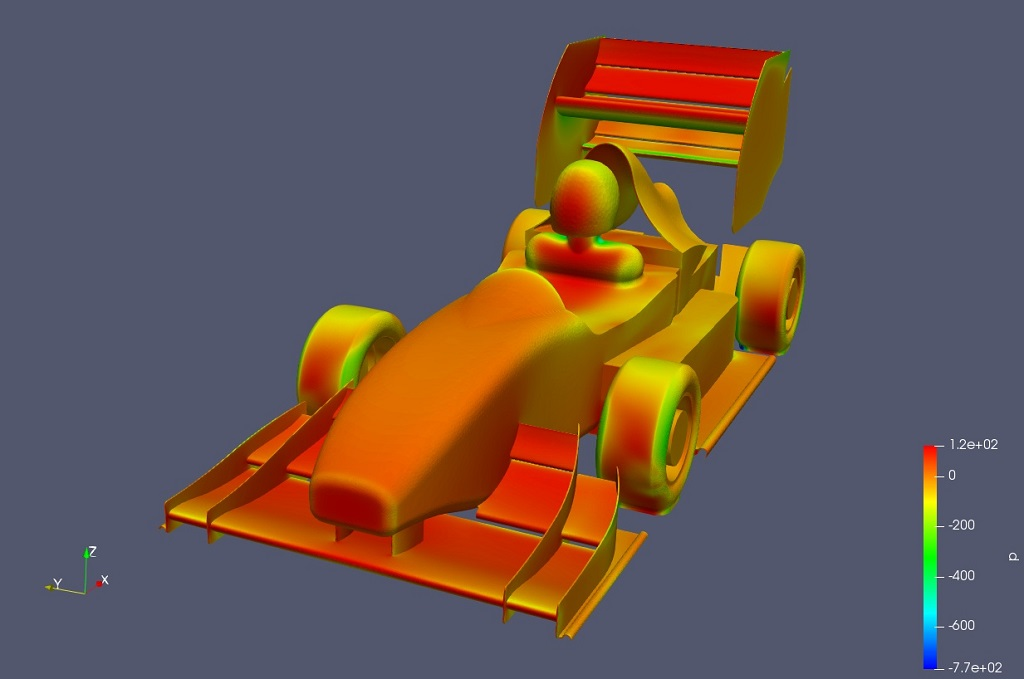
\includegraphics[width=\textwidth]{cis.jpg}
    %\caption{Pressure}
    \end{subfigure}
    \begin{subfigure}[b]{0.48\textwidth}
    	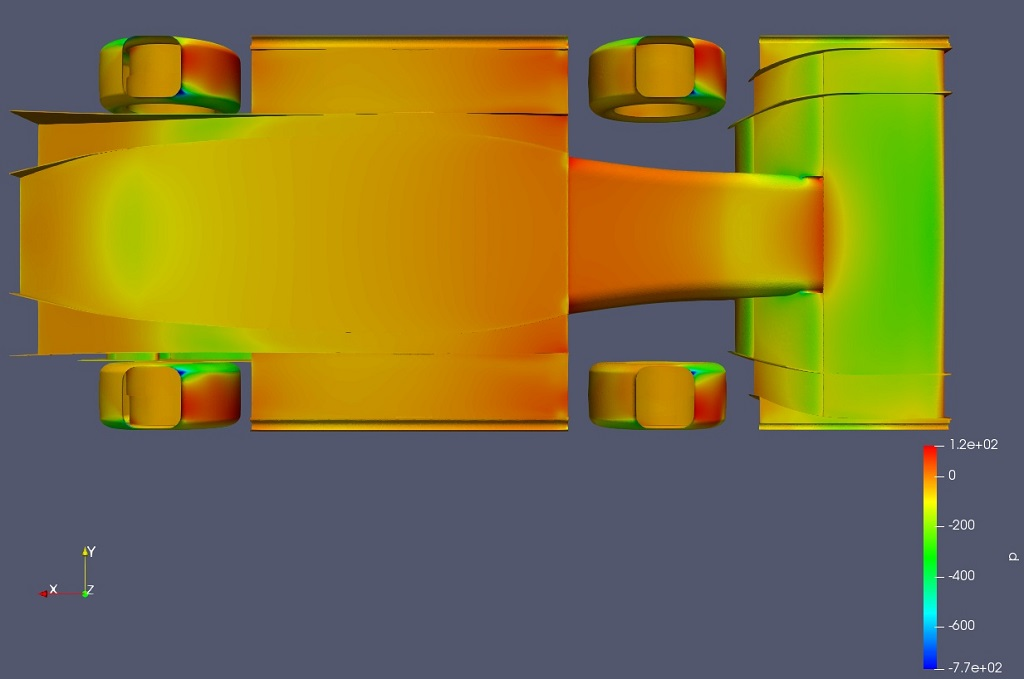
\includegraphics[width=\textwidth]{cis2.jpg}
        %\caption{Pressure}
    \end{subfigure}
    \begin{subfigure}[b]{0.48\textwidth}
    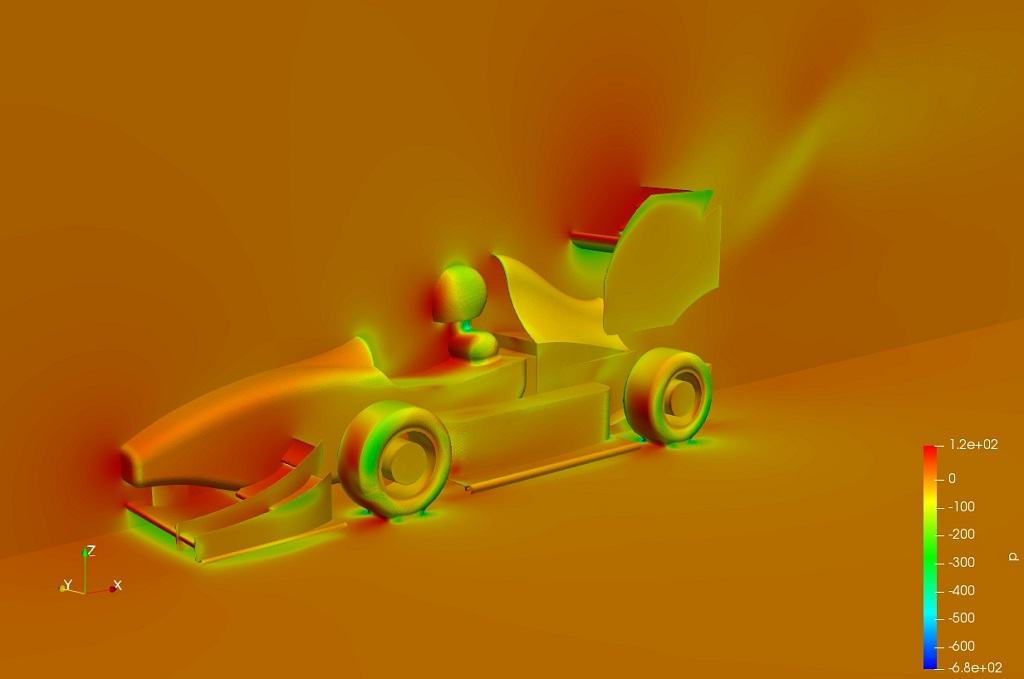
\includegraphics[width=\textwidth]{cis3.jpg}
    %\caption{Pressure}
    \end{subfigure}
    \begin{subfigure}[b]{0.48\textwidth}
    	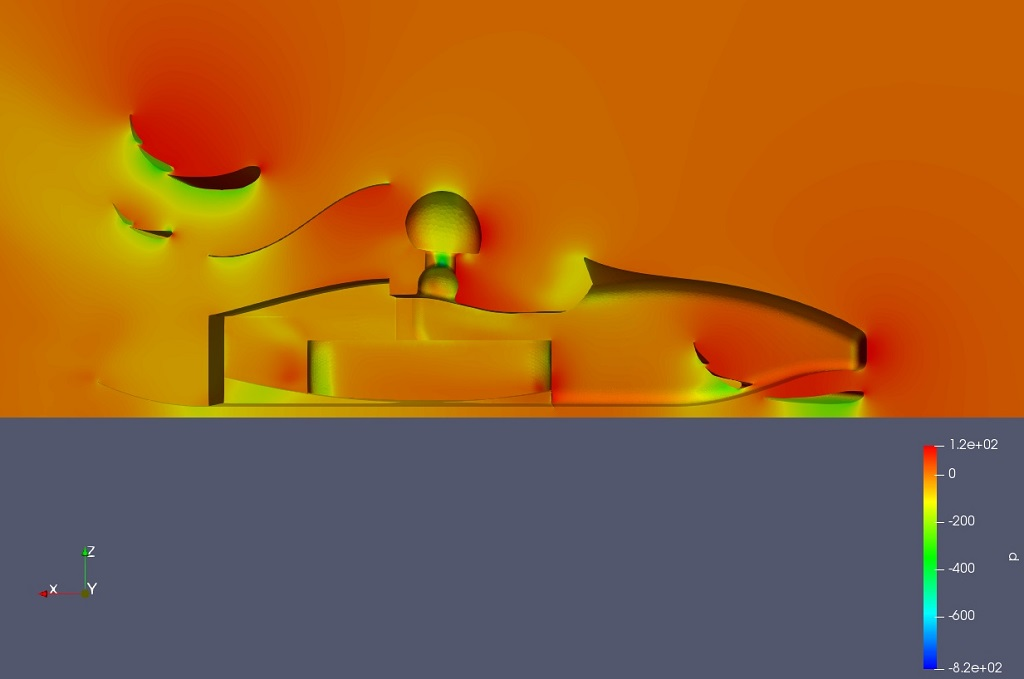
\includegraphics[width=\textwidth]{cis_sym.jpg}
        %\caption{Pressure}
    \end{subfigure}
    \caption{Contours of pressure}
    \begin{subfigure}[b]{0.7\textwidth}
    \centering
    	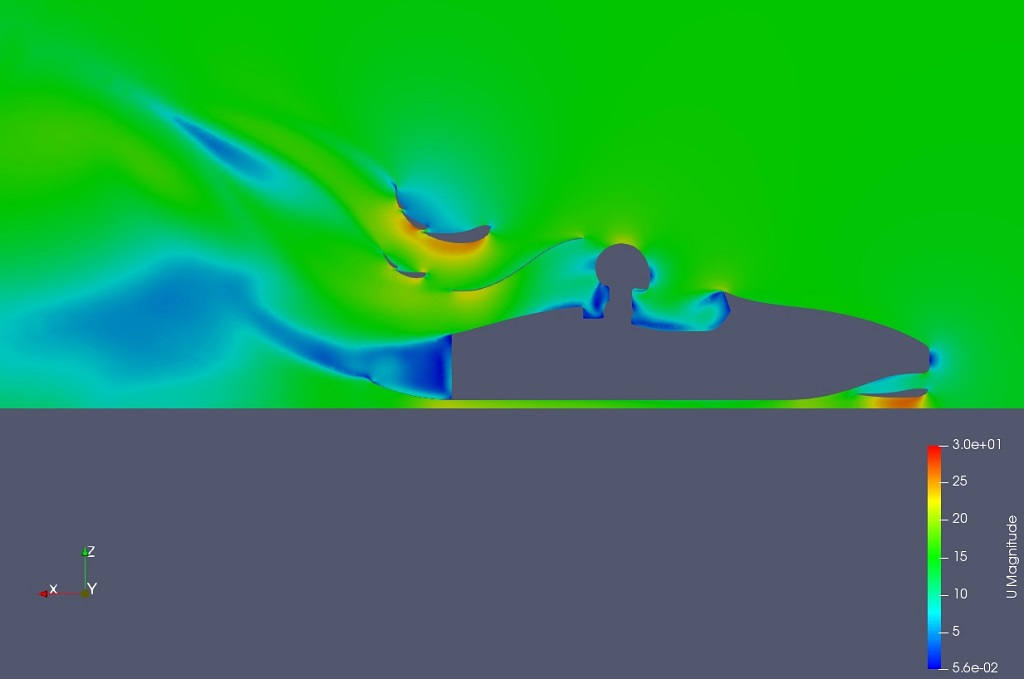
\includegraphics[width=0.7\textwidth]{vel.jpg}
    \end{subfigure}
    \caption{Contours of velocity}
\end{figure}

\newpage
Good visualization of the flow are streamlines which show, how air flow over (and under) the car. They give many information and they help improving the construction. 
\begin{figure}[h!]
	\centering
    \begin{subfigure}[b]{0.49\textwidth}
    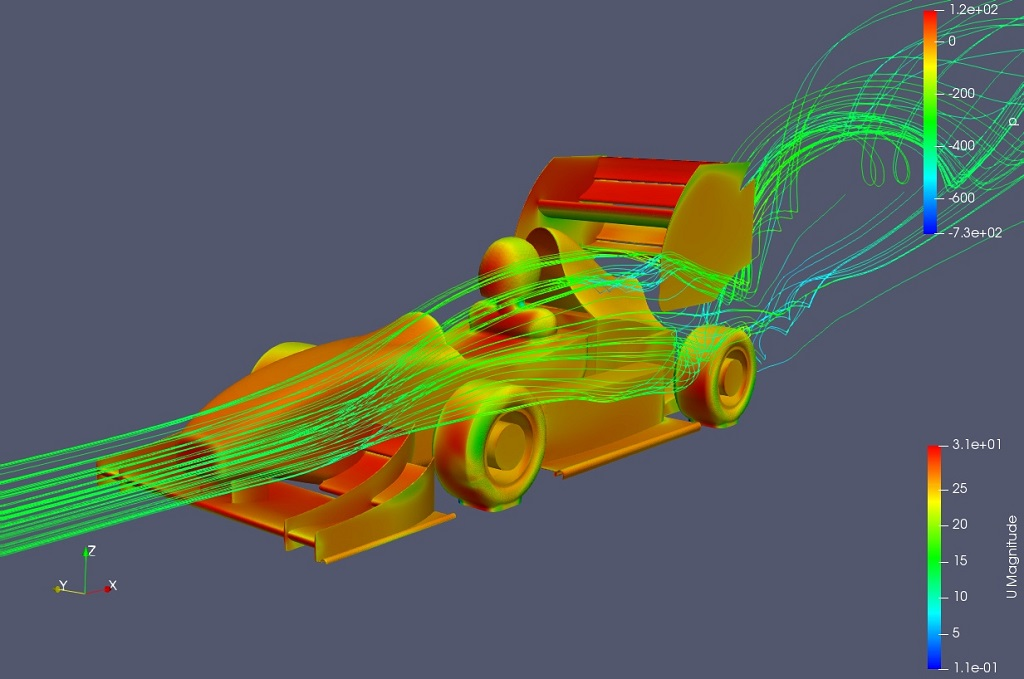
\includegraphics[width=\textwidth]{linie.jpg}
    %\caption{}
    \end{subfigure}
    \begin{subfigure}[b]{0.49\textwidth}
    	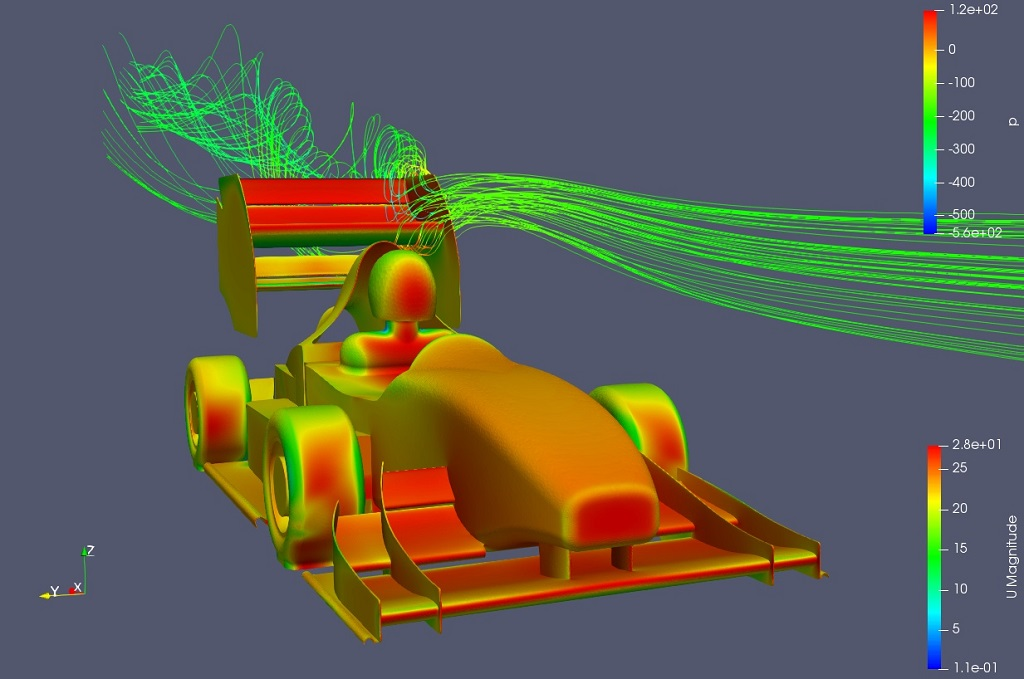
\includegraphics[width=\textwidth]{linie2.jpg}
        %\caption{}
    \end{subfigure}
    \begin{subfigure}[b]{0.49\textwidth}
    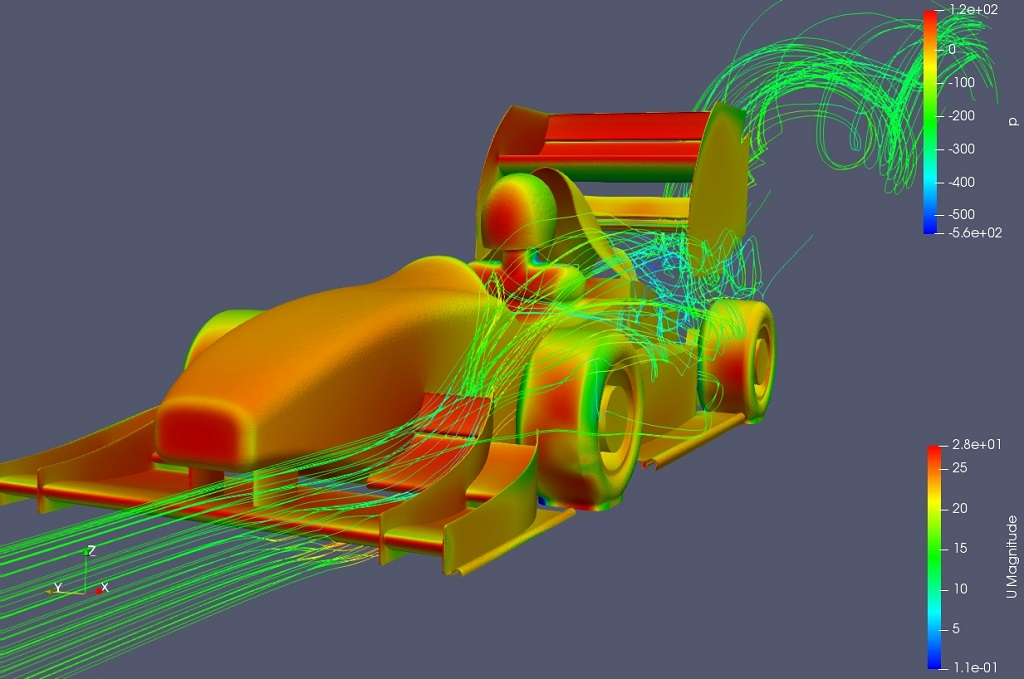
\includegraphics[width=\textwidth]{linie3.jpg}
    %\caption{}
    \end{subfigure}
    \begin{subfigure}[b]{0.49\textwidth}
    	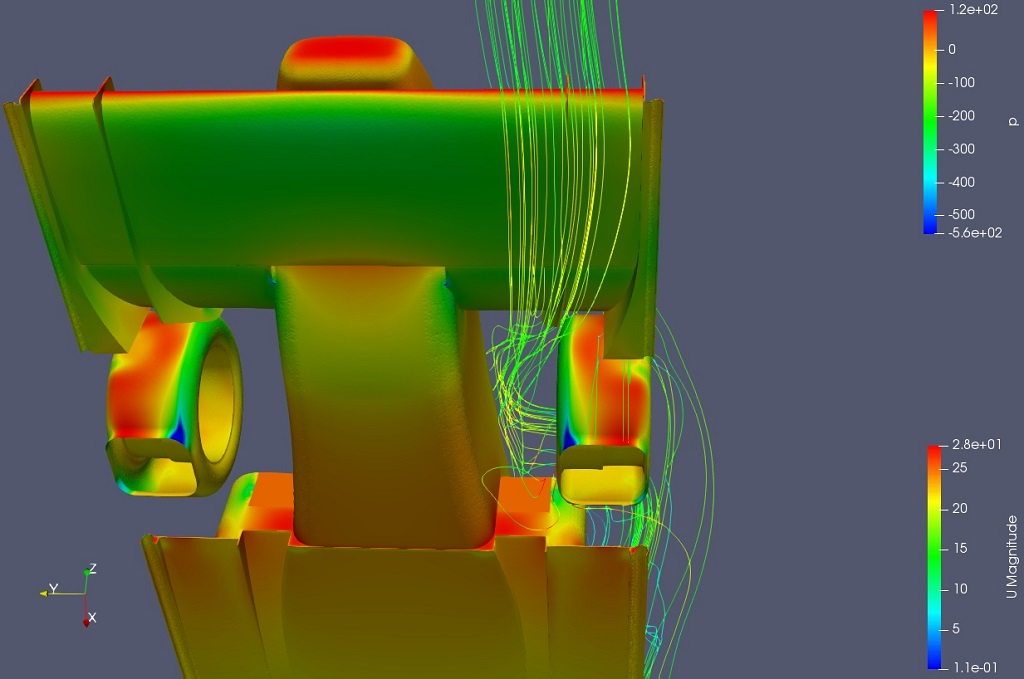
\includegraphics[width=\textwidth]{linie4.jpg}
        %\caption{}
    \end{subfigure}
    \caption{Streamlines}
   
\end{figure}


\subsection{Comparison with Fluent}
The same calculation has been carried out in Fluent, one of the best CFD software. Is OpenFoam, as open source, free software, as good as commercial software? The down forces and coefficients will be compared:

\begin{tabular}{lr|c|c}
Patch		&	OpenFoam		&	Fluent		&Difference\\\hline
Rear Wing	&-178N				&-186N			&4\%\\
Front Wing	&-132N				&-156N			&15\%\\
Diffuser	&-112N				&-98N			&-14\%\\
Others		&92N				&102N			&-10\%\\\hline
Sum			&-330N				&-338N			&2\%\\\hline\hline
Cl			&-2,11				&-1,9			&-11\%\\
Cx			&0,87				&0,95			&-8\%\\

\end{tabular}

Differences are about 10\% between OpenFoam and Fluent. It is quite a lot. The reason may be in low mesh quality and not enough elements. 